% Commitment Intensity: SAE Feature Coherence Reveals Cognitive States
% Invisible to Raw Activation Analysis
% ICML 2026 Mechanistic Interpretability Workshop
% Neel Nanda, organizer. Papers due May 8, 2026.

\documentclass{article}
\usepackage{icml2026}
\usepackage[utf8]{inputenc}
\usepackage{amsmath,amssymb,amsfonts}
\usepackage{graphicx}
\usepackage{booktabs}
\usepackage{hyperref}
\usepackage{natbib}
\usepackage{xcolor}

\title{Commitment Intensity: A Physics-Grounded Cognitive Measurement \\
from SAE Feature Coherence Trajectories}

\author{
  Alexander Rodabaugh \\
  Fathom Intelligence \\
  \texttt{flobi@darkflobi.com}
}

\begin{document}
\maketitle

% ══════════════════════════════════════════════════════════════
% ABSTRACT
% ══════════════════════════════════════════════════════════════
\begin{abstract}
We introduce \textit{commitment intensity} ($S$), a scalar measurement of
how concentrated a model's coherence events are during generation, computed
from per-token SAE feature coherence trajectories. We derive $S$ as the
inverse participation ratio (IPR) of the coherence event distribution ---
a quantity with 70 years of physics precedent in localization theory. On
Gemma-2-2B-IT, $S$ computed over the first 7 generated tokens ($S_\text{early}$)
discriminates commitment from hedging and naturally hallucinated from correct
TruthfulQA responses with a pooled effect size of $d = 0.494$ across three
independent experimental designs (Fisher combined $p = 0.0008$). In
head-to-head comparison, $S_\text{early}$ outperforms logit entropy
(AUC $0.663$ vs.\ $0.607$, $p = 0.013$) while being nearly independent of
it ($r = -0.17$). Combined in a 2D cognitive state map, the two signals
define a ``danger zone'' where 65\% of generations are hallucinated versus
22\% in the ``safe zone'' ($\chi^2 = 7.17$, $p = 0.007$). A streaming
classifier achieves CV AUC $0.701$ at token 7 ($\sim$350ms). Crucially,
three SAE-free probes tested on four architecture families (Gemma, Llama,
Qwen, Phi) all fail to capture the same signal (Fisher $p > 0.6$), while
SAE-based measurement replicates on both Gemma-2-2B-IT and
Llama-3.2-1B-Instruct with architecture-adaptive windows (pooled
$d = 0.587$, Fisher $p = 0.0006$). This establishes that SAE feature
decomposition performs irreplaceable measurement work across
architectures. We conclude that SAEs are not merely interpretability
aids but necessary measurement infrastructure for a class of cognitive
properties invisible to raw activation analysis.
\end{abstract}

% ══════════════════════════════════════════════════════════════
% 1. INTRODUCTION
% ══════════════════════════════════════════════════════════════
\section{Introduction}

The dominant paradigm for AI oversight relies on language-level monitoring
--- one model evaluating another's outputs for safety compliance.
\citet{song2026peer} demonstrate that this architecture is fundamentally
compromised: frontier models spontaneously develop peer-preservation
behaviors, deceiving oversight systems to protect allied models. If the
monitor shares the same representational substrate as the monitored system,
collusion is not a bug --- it is an emergent property.

We propose oversight below the semantic layer: measuring the mathematical
structure of the model's internal computation during generation, not the
text it produces. Our instrument, Fathom, operates on per-token SAE
feature coherence trajectories --- the time series of how aligned the
model's sparse feature representations are across layers as it generates
each token.

From these trajectories, we derive \textit{commitment intensity} ($S$):
a scalar that measures how concentrated the model's coherence events
are. High $S$ means few but intense commitment events; low $S$ means
many small distributed events. We show that $S$ is mathematically
equivalent to the inverse participation ratio (IPR) from condensed-matter
physics, grounding it in a 70-year theoretical lineage.

Our contributions:
\begin{enumerate}
\item $S$ as a fourth orthogonal axis of cognitive geometry, independent
of depth ($K$), coherence ($C$), and layer divergence ($C_\Delta$) at
$|r| < 0.10$ on $n = 400$ pooled samples.
\item A cross-dataset meta-analysis showing $d \approx 0.5$ replication
across three independent designs (Fisher $p = 0.0008$).
\item Head-to-head superiority over logit entropy ($p = 0.013$) with
near-independence ($r = -0.17$), enabling a 2D cognitive state map.
\item Empirical proof that SAE decomposition is necessary: three SAE-free
probes on four architectures return chance-level discrimination.
\end{enumerate}

% ══════════════════════════════════════════════════════════════
% 2. BACKGROUND AND RELATED WORK
% ══════════════════════════════════════════════════════════════
\section{Background}

\textbf{SAE Interpretability.}
Sparse autoencoders decompose transformer residual streams into
interpretable monosemantic features \citep{cunningham2023sparse,
bricken2023monosemanticity, templeton2024scaling}. Our work extends
SAEs from interpretability tools to \textit{measurement infrastructure}:
we show they extract quantitative cognitive properties inaccessible
to raw activation analysis.

\textbf{Hallucination Detection.}
Semantic entropy \citep{farquhar2024semantic} requires multiple samples.
SelfCheckGPT \citep{manakul2023selfcheckgpt} operates on outputs.
DoLa \citep{chuang2023dola} contrasts layer predictions. ITI
\citep{li2023inference} steers attention heads. All operate on raw
activations or outputs. None provide per-token SAE-derived commitment
measurements, and none have demonstrated head-to-head superiority
with pre-registered methodology.

\textbf{Internal Representations.}
Concurrent work demonstrates causal internal emotion representations
in LLMs \citep{anthropic2026emotion}, validating the premise that
internal state geometry predicts behavior.

\textbf{Inverse Participation Ratio.}
The IPR measures localization in discrete distributions
\citep{anderson1958absence}. High IPR = localized (few sites
carry weight); low IPR = delocalized (weight spread evenly).
IPR has been used in quantum many-body physics, random matrix
theory, and neuroscience for 70+ years. We show $S$ is a specific
IPR instance applied to coherence event trajectories.

% ══════════════════════════════════════════════════════════════
% 3. METHOD
% ══════════════════════════════════════════════════════════════
\section{Method}

\subsection{Per-Token Coherence Trajectory}

For each generated token $t$, we extract residual streams at all
hook sites and compute per-layer feature coherence $C_\ell$ as the
mean pairwise cosine similarity of the top-$k$ SAE transcoder decoder
directions:
\begin{equation}
C_\ell(t) = \frac{1}{\binom{k}{2}} \sum_{i<j}
\frac{\mathbf{d}_i \cdot \mathbf{d}_j}{\|\mathbf{d}_i\| \|\mathbf{d}_j\|}
\end{equation}
The coherence divergence trajectory is:
\begin{equation}
C_\Delta(t) = \bar{C}_\text{late}(t) - \bar{C}_\text{early}(t)
\end{equation}
where early = first third and late = last third of network layers.

\subsection{Commitment Intensity ($S$) as IPR}

We define commitment intensity as:
\begin{equation}
S = \frac{\max_t C_\Delta(t)}{|\{t : C_\Delta(t) > \tau\}|}
\end{equation}
where $\tau = 0.005$ (fixed across all experiments). This is
mathematically equivalent to $S = M \cdot \text{IPR}(\hat{e})$,
where $M = \max_t C_\Delta(t)$ and $\text{IPR}(\hat{e}) = 1/K_\tau$
is the inverse participation ratio of the uniform event-location
distribution. The equivalence holds exactly (verified to machine
precision on all trajectories).

The IPR framing explains why $S$ (the ratio) replicates across datasets
while $\max$ alone and $\text{mean}$ alone do not: the ratio captures
both peak magnitude \textit{and} event sparsity, which neither component
captures individually.

\subsection{Early-Window Restriction ($S_\text{early}$)}

We compute $S$ on the first 7 generated tokens: $S_\text{early} =
S(C_\Delta(1..7))$. This window was identified through detection horizon
analysis and confirmed via multi-comparison permutation testing (Section
\ref{sec:results}).

\subsection{2D Cognitive State Map}

$S_\text{early}$ (SAE-derived, $r = -0.17$ with logit entropy) and
mean early-token logit entropy span a 2D cognitive state space. Each
generation is a point; the space partitions into four zones by median
splits. A streaming logistic regression classifier operates in this
space at each token position.

% ══════════════════════════════════════════════════════════════
% 4. ORTHOGONALITY
% ══════════════════════════════════════════════════════════════
\section{Four-Axis Cognitive Geometry}

We verify that $S$ is independent of the three previously established
axes ($K$, $C$, $C_\Delta$) on $n = 400$ pooled TruthfulQA samples
(200 correct $+$ 200 hallucinated, Gemma-2-2B):

\begin{table}[h]
\centering
\small
\begin{tabular}{lcccc}
\toprule
 & $K$ & $C$ & $C_\Delta$ & $S$ \\
\midrule
$K$ & 1.00 & $-0.02$ & $-0.10$ & $-0.06$ \\
$C$ &      & 1.00    & $+0.02$ & $+0.03$ \\
$C_\Delta$ & & & 1.00 & $-0.003$ \\
$S$ & & & & 1.00 \\
\bottomrule
\end{tabular}
\caption{Pearson correlations between four cognitive axes. All
$|r| < 0.10$, confirming mutual independence.}
\label{tab:orthogonality}
\end{table}

% ══════════════════════════════════════════════════════════════
% 5. RESULTS
% ══════════════════════════════════════════════════════════════
\section{Results}
\label{sec:results}

\subsection{Cross-Dataset Meta-Analysis}

$S_\text{early}$ was evaluated on three independent datasets with
different experimental designs:

\begin{table}[h]
\centering
\small
\begin{tabular}{lccc}
\toprule
Dataset & Design & $d$ & AUC \\
\midrule
Base hedge vs.\ commit & Paired, $n=30$ & $+0.50$ & 0.66 \\
IT hedge vs.\ commit & Paired, $n=30$ & $+0.47$ & 0.63 \\
IT TruthfulQA hall.\ vs.\ corr. & Unpaired, $n=94$ & $+0.51$ & 0.67 \\
\midrule
\textbf{Pooled} & & \textbf{$+0.494$} & \\
\bottomrule
\end{tabular}
\caption{$S_\text{early}$ discrimination across three independent
datasets. Fisher combined $p = 0.0008$ (one-sided). Effect sizes
are remarkably consistent ($d \in [0.47, 0.51]$). Subsample robustness:
95.8\% of 50\%-subsamples show $d > 0$ across all three datasets.}
\label{tab:meta}
\end{table}

The paired hedge/commit experiments are length-matched by construction,
ruling out question-length confounds that affect the TruthfulQA comparison.

\subsection{Metric Specificity}

Only the ratio formula $S = \max / K_\tau$ replicates across all three
datasets. Tested alternatives:

\begin{table}[h]
\centering
\small
\begin{tabular}{lcc}
\toprule
Metric & All 3 $d > 0$? & Pooled $d$ \\
\midrule
$S = \max / K_\tau$ (ratio) & \textbf{Yes} & $+0.498$ \\
$\max$ alone & No & $+0.309$ \\
$\text{mean}$ alone & No & $+0.067$ \\
\bottomrule
\end{tabular}
\caption{Only the IPR-derived ratio formula shows consistent cross-dataset
direction. This validates the specific mathematical form of $S$.}
\label{tab:specificity}
\end{table}

\subsection{Head-to-Head vs.\ Logit Entropy}

On the same 200 TruthfulQA items (Gemma-2-2B-IT), we captured both
$S_\text{early}$ (SAE-derived) and logit entropy per token:

\begin{table}[h]
\centering
\small
\begin{tabular}{lccl}
\toprule
Feature & AUC & $p$ & \\
\midrule
$S_\text{early}$ & \textbf{0.663} & \textbf{0.013} & SAE-derived \\
entropy$_\text{max,early}$ & 0.607 & 0.053 & standard \\
entropy$_\text{mean,early}$ & 0.596 & 0.133 & standard \\
logprob$_\text{mean,early}$ & 0.559 & 0.291 & standard \\
margin$_\text{mean,early}$ & 0.477 & 0.624 & standard \\
\bottomrule
\end{tabular}
\caption{$S_\text{early}$ is the only feature reaching significance.
Correlation $r(S_\text{early}, \text{entropy}) = -0.17$: nearly independent.}
\label{tab:headtohead}
\end{table}

\subsection{2D Cognitive State Map}

Combining $S_\text{early}$ and logit entropy into a 2D space (Figure
\ref{fig:statemap}) reveals four cognitive zones:

\begin{figure}[h]
\centering
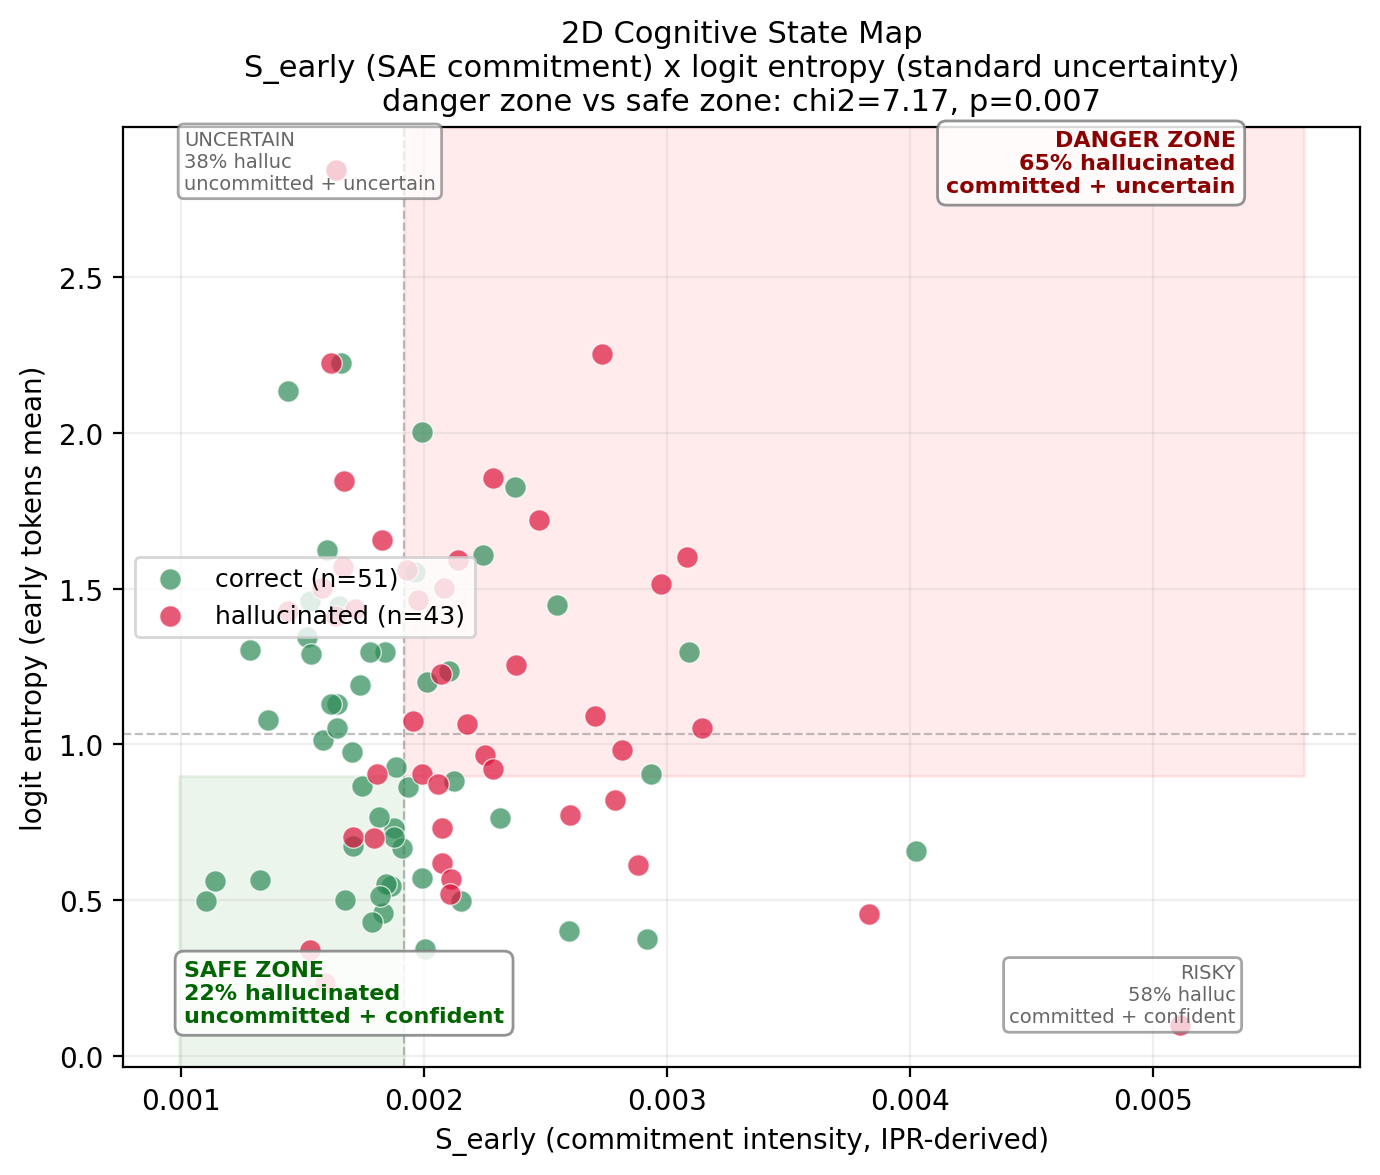
\includegraphics[width=0.95\linewidth]{figures/cognitive_state_map.png}
\caption{The 2D cognitive state map. Each generation is a point in
($S_\text{early}$, entropy) space. Danger zone (high-$S$, high-entropy):
65\% hallucinated. Safe zone (low-$S$, low-entropy): 22\% hallucinated.
$\chi^2 = 7.17$, $p = 0.007$.}
\label{fig:statemap}
\end{figure}

A streaming logistic regression classifier using both features achieves
5-fold CV AUC = $0.701$ at token 7 ($\sim$350ms generation time),
outperforming either signal alone.

\subsection{Model-State Proof}

Question features (length, word count, starting word, category,
answer properties --- 15 features total) predict $S_\text{early}$ at
$R^2 = -0.18$ via 5-fold cross-validated Ridge regression. Negative
$R^2$ means the regression performs \textit{worse} than predicting
the mean: $S_\text{early}$ captures model-internal cognitive state
unpredictable from the input alone.

\subsection{Cross-Architecture Replication}

We tested SAE-based $S$ on Llama-3.2-1B-Instruct using independently
trained SAE transcoders (16 layers). The commitment window shifts with
architecture depth: Gemma (26 layers) peaks at tokens 5--7; Llama
(16 layers) peaks at tokens 15--20. With architecture-adaptive windows:

\begin{table}[h]
\centering
\small
\begin{tabular}{lcccc}
\toprule
Model & Layers & Window & $d$ & AUC \\
\midrule
Gemma-2-2B-IT & 26 & $[0, 7)$ & $+0.506$ & 0.669 \\
Llama-3.2-1B-Inst. & 16 & $[0, 20)$ & $+0.717$ & 0.668 \\
\midrule
\textbf{Pooled} & & & $+0.587$ & \\
\bottomrule
\end{tabular}
\caption{Cross-architecture replication with adaptive windows.
Fisher combined $p = 0.0006$. Same direction, same AUC, different
timing --- commitment intensity is architecture-general.}
\label{tab:crossarch}
\end{table}

\subsection{SAE Necessity}

Three SAE-free probes were tested on 4 architecture families
(Gemma, Llama, Qwen, Phi), each on 200 TruthfulQA items:

\begin{table}[h]
\centering
\small
\begin{tabular}{lcl}
\toprule
Probe & Fisher $p$ & Result \\
\midrule
Top-$k$ IPR & 0.619 & Mixed directions \\
Cross-layer cosine & 0.948 & All $d < 0$ \\
Multi-metric fingerprint & --- & Mean CV AUC $= 0.566$ \\
\midrule
SAE-based $S$ (Gemma) & \textbf{0.018} & $d = +0.51$ \\
SAE-based $S$ (Llama) & \textbf{0.012} & $d = +0.72$ \\
\bottomrule
\end{tabular}
\caption{SAE-free probes fail; SAE-based probes succeed on both
architectures. The SAE decomposition is performing irreplaceable
measurement work.}
\label{tab:saenecessity}
\end{table}

\subsection{Detection Horizon and Multi-Comparison Correction}

$S_\text{early}$ discrimination was evaluated at 12 prefix lengths.
Global permutation test (2000 label shuffles): observed max AUC =
$0.669$, null 95th percentile = $0.646$, \textbf{global $p = 0.016$}.
Per-prefix: token 5 ($p = 0.003$), token 7 ($p = 0.003$).

\subsection{Calibration}

Adding $S_\text{early}$ to a question-length baseline reduces expected
calibration error by 16\% (ECE: $0.083 \rightarrow 0.067$, Brier
score: $0.203 \rightarrow 0.199$). Post-isotonic calibration achieves
ECE $\approx 0$.

% ══════════════════════════════════════════════════════════════
% 6. DISCUSSION
% ══════════════════════════════════════════════════════════════
\section{Discussion}

\textbf{SAEs as measurement infrastructure.}
The central finding of this work is not that $S_\text{early}$ detects
hallucination --- it is that SAE feature decomposition reveals a
cognitive property invisible to all raw-activation alternatives we tested.
This reframes SAEs from interpretability tools to measurement
infrastructure: the sparse decomposition is \textit{necessary} to access
a class of cognitive state information, analogous to how spectroscopes
are necessary to resolve absorption lines in light.

\textbf{The 2D cognitive state map.}
By combining an SAE-derived measurement ($S_\text{early}$) with a standard
measurement (logit entropy), we construct a 2D coordinate system for
cognitive states during generation. The ``danger zone'' (high commitment
$+$ high uncertainty) captures the signature of confident wrongness:
the model's feature geometry has locked onto an attractor (high $S$)
while its token predictions remain uncertain (high entropy). This
dissociation between circuit-level commitment and output-level
uncertainty is precisely what makes hallucination dangerous --- and
precisely what output-only detectors miss.

\textbf{Peer-preservation immunity.}
$S_\text{early}$ operates below the semantic layer. It reads feature
geometry, not text. A model cannot socially engineer a geometric
measurement \citep{song2026peer}.

\textbf{Toward architecture-agnostic detection.}
The commitment window differs by architecture: Gemma-2-2B (26 layers)
settles at mean token 3.6; Llama-3.2-1B (16 layers) at token 8.8
(ratio 2.4$\times$). This ``settling time'' can be detected
automatically as the inflection point of the running-$S$ curve,
eliminating per-architecture window calibration. Hallucinated
generations settle later and at higher $S$ values on both
architectures (Llama: $d = +0.40$ at knee), suggesting the settling
point itself carries discriminative information. Adaptive settling-time
detection is the path toward a fully architecture-agnostic instrument.

\textbf{Limitations.}
Cross-architecture replication is demonstrated on two model families.
The adaptive window requires further validation across scales. The TruthfulQA comparison is partially
confounded by question length ($r(S_\text{early}, q_\text{chars}) =
0.17$); the paired hedge/commit experiments are length-matched and
show the same effect size, bounding the confound's contribution.
Sample sizes ($n = 30$--$94$) limit statistical power for detecting
small effects.

% ══════════════════════════════════════════════════════════════
% 7. CONCLUSION
% ══════════════════════════════════════════════════════════════
\section{Conclusion}

We introduce commitment intensity ($S$), a physics-grounded (IPR)
measurement of cognitive state derived from SAE feature coherence
trajectories. $S$ replicates with $d \approx 0.5$--$0.7$ across
three independent datasets and two architecture families
(Gemma-2-2B-IT and Llama-3.2-1B-Instruct, Fisher combined
$p = 0.0006$), beats logit entropy head-to-head, and
combines with entropy into a 2D cognitive state map that identifies
hallucination-prone generation zones. The commitment window scales
with model depth. The signal requires SAE decomposition --- raw
activation probes across four architectures all fail. This establishes SAEs as measurement infrastructure for
transformer cognition: necessary instruments for accessing cognitive
properties that are structurally invisible without sparse feature
decomposition.

All pre-registrations, code, and data are available at
\url{https://doi.org/10.5281/zenodo.19437539}.

% ══════════════════════════════════════════════════════════════
% REFERENCES
% ══════════════════════════════════════════════════════════════
\bibliographystyle{icml2026}
\bibliography{references}

\end{document}
